\documentclass[a4paper,11pt]{article}
\usepackage{graphicx,url}
\usepackage[T1]{fontenc}
\usepackage[utf8]{inputenc}
\usepackage[brazil]{babel}
\usepackage{a4wide}
\graphicspath{{./imagens/}}
\title{\vspace{-4cm}Relatório 02 - Laboratório de Arquitetura de Computadores}
\author{Luiz Junio Veloso Dos Santos - Matricula: 624037}

\begin{document} 

\maketitle

\begin{enumerate} 
    \item \textbf{Circuito no Simulador 97:}
        \begin{figure}[ht]
            \caption{Somador completo CLA de 4 bits }
            \centering
            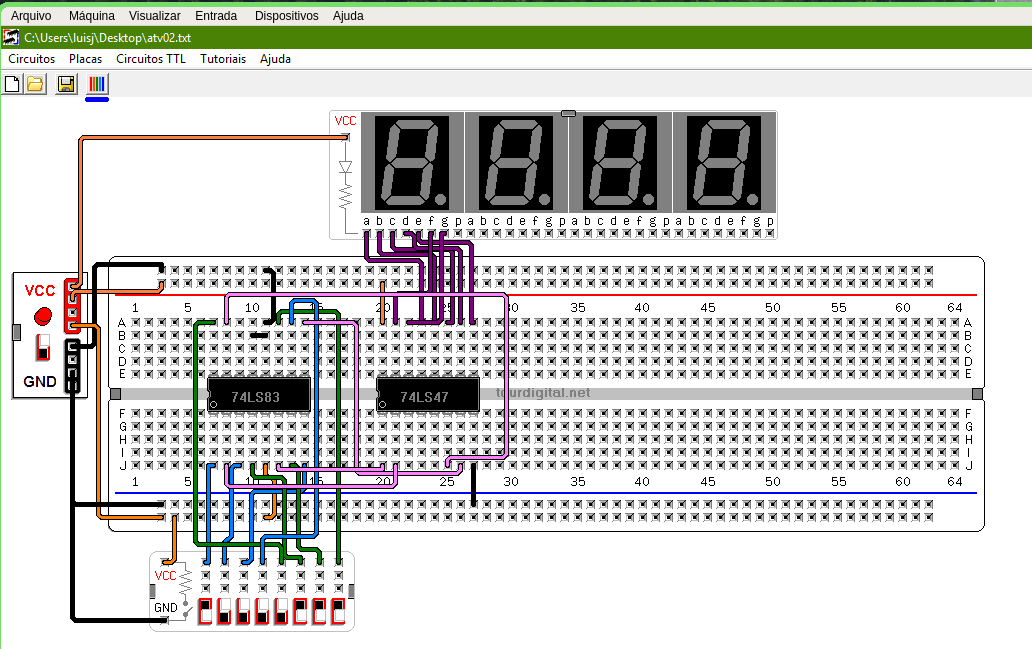
\includegraphics[width=17cm]{somadorCompleto97.png}
        \end{figure}
        \newpage
    \item \textbf{Circuitos no Logisim:}
        \begin{figure}[ht]
            \caption{Somador CLA de 4 bits}
            \centering
            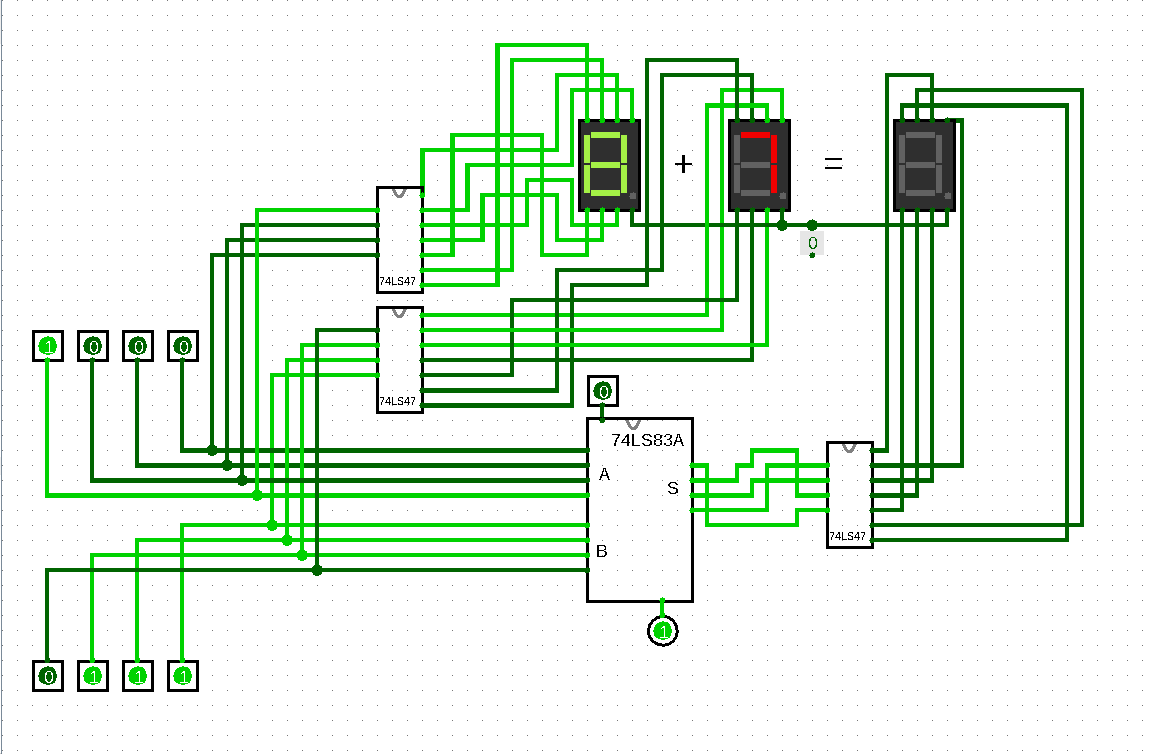
\includegraphics[width=17cm]{somadorCLA-logisim}
        \end{figure}
        \newpage
        \begin{figure}[ht]
            \caption{74LS83A}
            \centering
            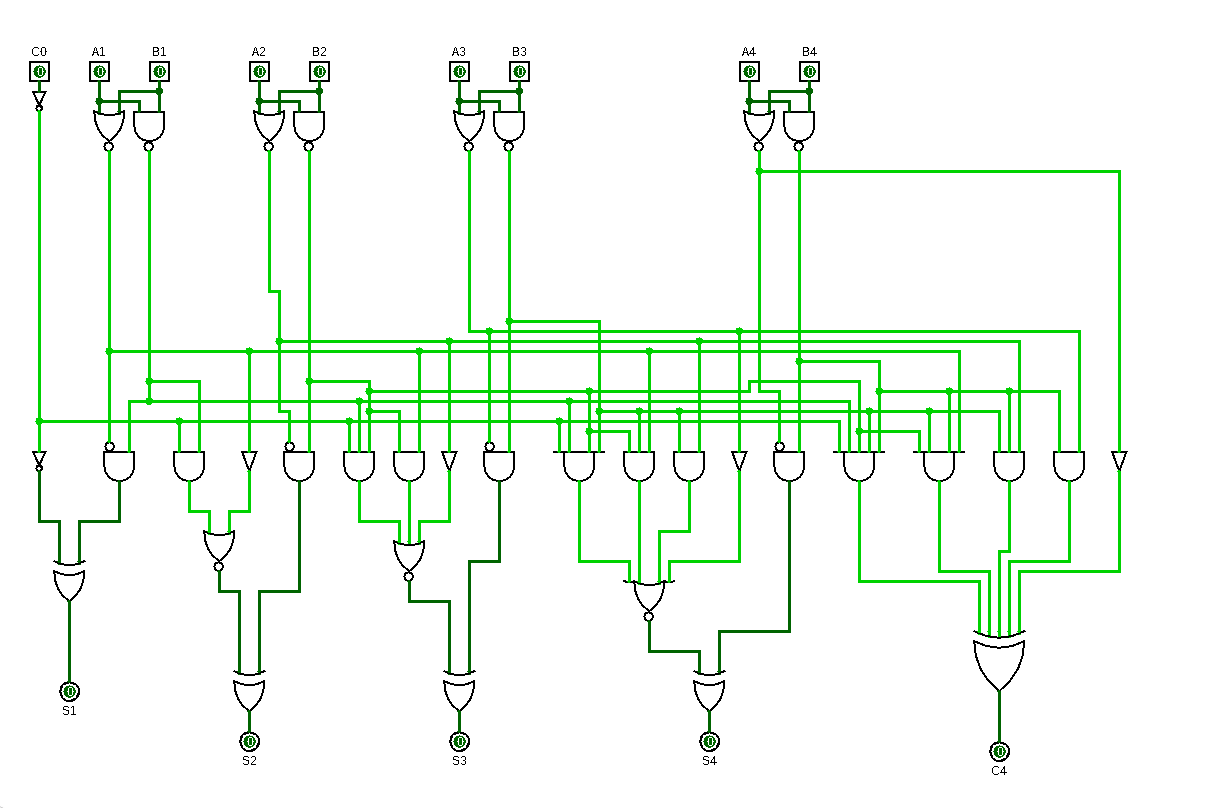
\includegraphics[width=16cm]{74LS83A}
        \end{figure}
        \newpage
        \begin{figure}[ht]
            \caption{74LS47 - Decodificador de 7 segmentos}
            \centering
            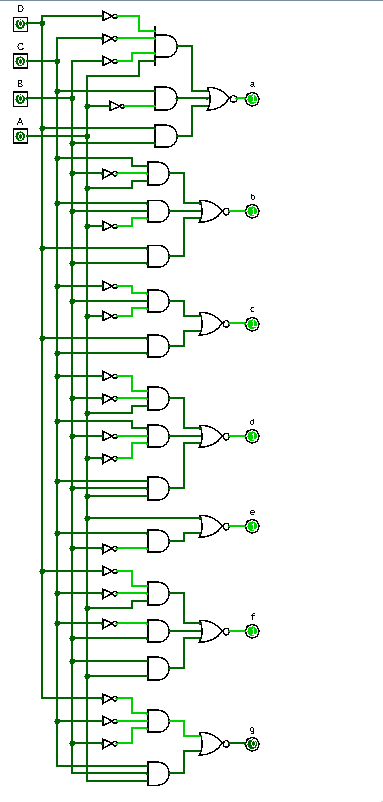
\includegraphics[width=10cm]{74LS47}
        \end{figure}
    
\end{enumerate}

\end{document}
